\subsection*{\center{Общая характеристика работы}}
Область исследований, с которой связана диссертация, является комплексной и включает в себя различные направления работ, в частности, создания различных интеллектуальных систем. Сфера применения интеллектуальных систем обширна, например, в Институте Чиная (Индия) Е. Джубилсоном и П. Дханавантини ведутся исследования интеллектуальных систем обработки запросов пользователей в области телекоммуникаций, а в университете Ганновера (Германия) Р. Брунс и Дж. Данкель разрабатывают интеллектуальные системы для обработки запросов в службу спасения с целью уменьшения времени реакции на происшествие. В Санкт-Петербургском государственном университете (СПбГУ) под руководством В.И. Золотарева проводится оценка эффективности службы информационной поддержки в Вычислительном центре СПбГУ. В Сингапуре С. Фу и П. Леонг проведен анализ эффективности ИТ-службы поддержки крупной компании и показана возможность автоматизации ряда процессов (ИТ~-- информационные технологии).\par
Исследования в области интеллектуальных систем повышения эффективности ИТ-службы предприятия ведутся также лидерами ИТ-отрасли: компаниями HP \footnote{Проект \url{https://en.wikipedia.org/wiki/HP_OpenView}} и IBM \footnote{Проект \url{http://www.ibm.com/smarterplanet/us/en/ibmwatson/}}. Например, известна многоцелевая интеллектуальная система IBM Watson, разработкой и исследованием которой занимается группа под руководством профессора А. Гоэля.  \par   
Для того чтобы система могла работать с запросами пользователя, она должна \quoted{понимать} язык, на котором они составлены. Подобные проблемы исследуются в области обработки естественного языка.  Например, это подход GATE \footnote{Проект \url{https://gate.ac.uk/}}, который активно развивается в университете Шеффилда (Великобритания) под руководством Г. Каллаган, Л. Моффат и С. Сзаз. Другое направление~--- это семантический поиск, исследования в этой области также активно ведутся в университете Шеффилда, в частности, разработан подход Mimir, который реализует возможности поиска по принципу «поиск и открытие». Для организации поиска решений в соответствии с запросами пользователей в таких системах используются онтологии, например, широко применяется подход, предложенный С. Дей и А. Джеймс из Калифорнийского университета (США), основанный на применении деревьев тегов в онтологии. \par
Для придания интеллектуальной системе гибкости необходимо дать ей возможность проводить логические рассуждения. Одной из ведущих организаций в этом направлении исследований является консорциум OpenCog \footnote{Проект \url{http://opencog.org/}} (США). Этими работами руководит Бен Герцель (председатель Artificial General Intelligence Society и OpenCog Foundation)~--- один из мировых лидеров в области искусственного интеллекта. Исследования в области машинной логики также ведутся в рамках проекта NARS \footnote{Проект \url{https://sites.google.com/site/narswang/}} под руководством профессора университета Темпла (США) Пея Вонга. \par 

\newcommand{\actuality}{\underline{\textbf{Актуальность темы.}}}
\newcommand{\aim}{{\textbf{Целью}}}
\newcommand{\tasks}{{\textbf{задачи}}}
\newcommand{\scope}{{\textbf{Область исследования}}}
\newcommand{\subject}{{\textbf{Предметом исследования}}}
\newcommand{\methods}{{\textbf{Методы исследования}}}
\newcommand{\defpositions}{{\textbf{Основные положения, выносимые на~защиту:}}}
\newcommand{\novelty}{{\textbf{Научная новизна}}}
\newcommand{\influence}{{\textbf{Практическая значимость.}}}
\newcommand{\reliability}{{\textbf{Достоверность}}}
\newcommand{\probation}{{\textbf{Апробация работы.}}}
\newcommand{\contribution}{{\textbf{Личный вклад.}}}
\newcommand{\publications}{{\textbf{Публикации.}}}


{\aim} работы является разработка интеллектуальной системы повышения эффективности деятельности ИТ-службы предприятия. \par
{\scope}~--- разработка методов и алгоритмов решения задач системного анализа, оптимизации, управления, принятия решений и обработки информации в ИТ-отрасли.\par
{\subject}  является процесс регистрации и устранения проблемных ситуаций, возникающих в ИТ-инфраструктуре предприятия.\par

Для достижения поставленной цели необходимо было решить следующие {\tasks}:
\begin{enumerate}
  \item Провести теоретико-множественный и теоретико-информационный анализ сложных систем в области поддержки информационной инфраструктуры;
  \item Создать модель целевой области;
  \item Исследовать модели мышления и выбрать наиболее подходящую;
  \item На основе выбранной модели мышления разработать модель проблемно-ориентированной системы управления, принятия решений и оптимизации процесса принятия, анализа и обработки запросов пользователя в области обслуживания информационной структуры предприятия;
  \item Создать архитектуру приложения на основе модели;
  \item Реализовать на основе этой архитектуры прототип интеллектуальной вопросно-ответной системы повышения эффективности деятельности ИТ-службы предприятия;
  \item Провести апробацию прототипа на тестовых данных.
\end{enumerate}

\defpositions
\begin{enumerate}
  \item Теоретико-множественный и теоретико-информационный анализ сложных систем в области поддержки информационной инфраструктуры;
  \item Построенная модель проблемно-ориентированной системы управления, принятия решений и оптимизации технических объектов в области обслуживания информационной инфраструктуры;
  \item Созданный прототип программной реализации модели проблемно-ориентированной системы управления, принятия решений и оптимизации обработки запросов пользователя в области обслуживания информационной инфраструктуры;
  \item Апробация прототипа проблемно-ориентированной системы управления, принятия решений и оптимизации деятельности на контрольных примерах и анализ ее результатов.
\end{enumerate}

\novelty проведенного исследования состоит в следующем:
\begin{enumerate}
  \item Создана модель проблемно-ориентированной системы управления, принятия решений в области обслуживания информационной структуры предприятия на основе модели мышления;
  \item Представлены новая модель данных для модели мышления и оригинальный способ хранения для этой модели, эффективный по сравнению с другими базами данных;
  \item Выполнено оригинальное исследование моделей мышления применительно к области обслуживания информационной структуры предприятия;
  \item На основе модели мышления Мински созданы архитектура системы обслуживания информационной структуры предприятия и программный прототип этой системы.
\end{enumerate}

\influence\ 
Система, разработанная в рамках данной диссертации носит значимый практический характер. Идея работы зародилась под влиянием производственных проблем в ИТ-отрасли, с которыми автор сталкивался каждый день в процессе разрешения различных инцидентов, возникающих в деятельности службы технической поддержки \icl~--- одном из крупнейших системообразующих предприятий ИТ-области Республике Татарстан. Поэтому было необходимо выработать глубокое понимание конкретной предметной области, чтобы выбрать приемлемое решение, получившее практическое применение в работе на проекте поддержки крупной сети продуктовых магазинов. \par
\reliability\ научных исследований и практических рекомендаций
базируется на корректной постановке общих и частных рассматриваемых задач,  использовании известных фундаментальных теоретических положений системного анализа, достаточном объёме данных, использованных при статистическом моделировании, и широком экспериментальном материале, использованном для численных оценок достижимых качественных показателей. \par 
Исследования, проведенные в диссертации, соответствуют паспорту специальности 05.13.01~--- Системный анализ, управление и обработка информации, сопоставление приведено в таблице \ref{ResearchDescription}.

\begin{longtable}{|p{7cm}|p{9cm}|}
 \caption[Сопоставление направлений исследований в рамках специальности 05.13.01 и исследований, проведенных в диссертации]{Сопоставление направлений исследований в рамках специальности 05.13.01 и исследований, проведенных в диссертации}\label{ResearchDescription} \\ 
 \hline
 
 \multicolumn{1}{|c|}{\textbf{Направление исследования}} & \multicolumn{1}{c|}{\textbf{Результат работы}}  \\ \hline 
\endfirsthead
\multicolumn{2}{c}%
{{\bfseries \tablename\ \thetable{} -- продолжение}} \\
\hline \multicolumn{1}{|c|}{\textbf{Направление исследования}} &
\multicolumn{1}{c|}{\textbf{Результат работы}}  \\ \hline 
\endhead

\hline \multicolumn{2}{|r|}{{Продолжение следует}} \\ \hline
\endfoot

\hline \hline
\endlastfoot
\hline
   Разработка критериев и моделей описания и оценки эффективности решения задач системного анализа, оптимизации, управления, принятия решений и обработки информации & В рамках работы была разработана модель системы принятия решения и обработки информации в области решения запросов пользователя на естественном языке. \\
   \hline
   Разработка проблемно-ориентированных систем управления, принятия решений и оптимизации технических объектов & По модели, разработанной в предыдущем пункте был разработан прототип системы принятия решения Thinking Understanding, который был испытан на модельных данных.\\
   \hline
   Методы получения, анализа и обработки экспертной информации & В рамках системы TU был разработан метод обработки экспертной информации - обучение при помощи модели мышления TU, основанной на принципах модели 6-ти Марвина Мински. \\
   \hline
   Разработка специального математического и алгоритмического обеспечения систем анализа, оптимизации, управления, принятия решений и обработки информации & В рамках разработки системы TU были созданы специальные алгоритмы для анализа запросов пользователя и принятия решений.\\
  \hline 
  Теоретико-множественный и теоретико-информационный анализ сложных систем & В рамках работы был проведен комплексный анализ области поддержки программного обеспечения, с помощью которого была построена система данной области и выделены участки для оптимизации принятия решений.\\
  \hline
  Методы и алгоритмы интеллектуальной поддержки при принятии управленческих решений в технических системах & Система, разработанная в рамках данной работы в включает в себя инновационные методы и алгоритмы поддержки принятия решений, использующих в своей основе модель мышления на базе модели мышления Человека, описанной в книге Марвина Мински. \\ 
  \hline
  Визуализация, трансформация и анализ информации на основе компьютерных методов обработки информации & Представлена наглядная визуализация данных по системному анализу области удаленной поддержки инфраструктуры. \\
  \hline	
\end{longtable}


\probation\
 Основные результаты диссертационной работы докладывались на следующих конференциях:
\begin{itemize}
	\item Десятая молодежная научная школа-конференция "Лобачевские чтения~---2011. Казань, 31 октября~--4 ноября 2011";
	\item 3rd World Conference on Information Technology (WCIT-2012); 
	\item Искусственный интеллект и естественный язык (AINL-2013);
	\item Электронная Казань~--- 2014;
	\item Электронные библиотеки: перспективные методы и технологии, электронные коллекции (RCDL-2014);
	\item Agents and multi-agent systems: technologies and applications (AMSTA-2015).
\end{itemize}
Практическая апробация результатов работы проводилась на выгрузке инцидентов из системы регистрации запросов службы технической поддержки ИТ-инфраструктуры \icl. Созданная система показала требуемые результаты (процент успешно обработанных запросов более чем 30\%) обработки данной информации.
\contribution\ Автор исследовал целевую область: проводил анализ запросов пользователей и классифицировал их, вместе с Талановым Максимом Олеговичем изучал модель мышления Марвина Мински; создавал базовую архитектуру систему; вместе с Талановым Максимом Олеговичем проводил разработку компонентов модели, адаптируя теорию Марвина Мински. Автор проводил испытание системы на целевых запросах; отлаживал работу системы.
\publications\ Основные результаты по теме диссертации изложены в 9 печатных изданиях  \cite{Lobachevskii},\cite{WCIT-2012},\cite{AINL-2013},\cite{ISGZ}, \cite{IJSE-1}, \cite{IJSE-2}, \cite{RCDL-2014}, \cite{AMSTA-2015}, \cite{VAK-1}, из которых статьи \cite{RCDL-2014},\cite{AMSTA-2015} проиндексированы в БД Scopus, статья \cite{AMSTA-2015} проиндексирована в БД Web Of Science, работа \cite{VAK-1} опубликована в журнале из списка ВАК, статья  \cite{ISGZ} проиндексирована в БД РИНЦ, работы \cite{Lobachevskii},\cite{WCIT-2012},\cite{AINL-2013},\cite{ISGZ} опубликованы в материалах международных и всероссийских конференций.



 % Характеристика работы по структуре во введении и в автореферате не отличается (ГОСТ Р 7.0.11, пункты 5.3.1 и 9.2.1), потому её загружаем из одного и того же внешнего файла, предварительно задав форму выделения некоторым параметрам

%Диссертационная работа была выполнена при поддержке грантов ...

%\underline{\textbf{Объем и структура работы.}} Диссертация состоит из~введения, четырех глав, заключения и~приложения. Полный объем диссертации \textbf{ХХХ}~страниц текста с~\textbf{ХХ}~рисунками и~5~таблицами. Список литературы содержит \textbf{ХХX}~наименование.

%\newpage
\subsection*{Содержание работы}
Во \textbf{введении} обоснована актуальность исследований, проведенных в рамках диссертации; даны общая характеристика работы и анализ исследований в области обслуживания информационной инфраструктуры предприятия; проведен обзор и на основе выявленного роста публикационной активности в рассматриваемой предметной области (по данным Scopus) обоснована актуальность проведенных исследований. \par

\textbf{Первая глава} диссертации посвящена постановке задачи и обзору интеллектуальных систем регистрации и анализа проблемных ситуаций, возникающих в ИТ-инфраструктуре предприятия.
Глава начинается с описания модели теории массового обслуживания (ТМО) для служб, занимающихся устранением проблемных ситуаций, возникающих в ИТ-инфраструктуре предприятия. На рисунке \ref{img:mass_service} представлена модель системы массового обслуживания, в которой использованы следующие обозначения: $\lambda$ --- интенсивность входящего потока;  $\alpha$ --- доля заявок, для которых время ожидания в очереди превышает $max(T_q)$;       
$\mu$ --- величина, обратная среднему времени нахождения заявки у агента;
$n$ --- число агентов;
$T_q$ --- время нахождение заявки в очереди в часах;
$SLA$ --- уровень обслуживания, ($1-\alpha$), доля заявок, для которых время в очереди не превышает $max(T_q)$: $T_p$ --- время удовлетворения заявки;
 $\alpha_n$ --- количество заявок;
 $T_{qp}=T_q+T_p$ --- время прохождения заявки через систему;
 $S(\mu)= \frac{R_p}{\mu} $ --- средняя стоимость выполнения одной заявки;
 $R_p$ --- средняя стоимость часа работы специалиста (выводится далее).

  
\begin{figure} [h] 
  \center
  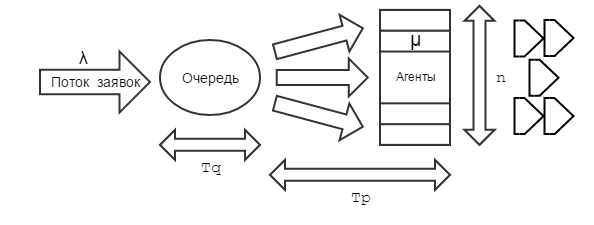
\includegraphics [scale=0.8] {mass_service}
  \caption{Модель системы массового обслуживания.} 
  \label{img:mass_service}  
\end{figure}

 
Существует несколько подходов решения задач ТМО: 
\begin{itemize}
	\item Аналитическое решение для простейших систем, которое позволяет выразить $T_q (t)$ через $\lambda$, $\mu$ и $n$;
	\item Решение с помощью имитационного подхода, где строится гистограмма $T_q (t)$, по которой оценивается достаточность $n$ для обеспечения SLA;
	\item Решение с помощью эконометрического подхода, которое подходит для систем с достаточно большим $n$. В таких системах возможно оценить $T_q (t)$ по имеющейся статистике.
\end{itemize} \par
На основе комбинации формул Эрланга, модели Энгсета и модели Полячека~--~Хинчина 
построена формула для решения задач ТМО на основе аналитического подхода путем нахождения распределения вероятностей для $T_{qp}$. Основной же задачей этой работы является прогнозирование необходимых ресурсов для максимизации $SLA$ ($SLA=1-\alpha$). 
В главе 1 диссертации рассмотрена задача минимизации $T_{qp}$, $S(\mu)$ и динамического выделения ресурсов. На основе  статистики, собранной в компании \icl,~ был подсчитан следующий коэффициент $T_{qp}=47,9$ при $n=6$; $SLA=0,82$; $\alpha=0,18$;  $\alpha_n=2920$.  \par

 В главе 1 также представлен сравнительный анализ систем регистрации и устранения проблемных ситуаций; определены основные требования к интеллектуальным системам регистрации и анализа проблемных ситуаций в ИТ-сфере. Одним из важных элементов подобных систем является обработка естественного языка, поэтому в данной главе представлен сравнительный анализ методов и программных комплексов обработки текстов. \par
При проведении анализа были использованы следующие средства обработки естественного языка: Open NLP\footnote{Проект \url{http://opennlp.apache.org}}, Relex\footnote{Проект \url{http://opencog.org}}, StanfordParser\footnote{Проект \url{http://nlp.stanford.edu/software/lex-parser.shtml}}.
Оценка качества функционирования этих средств проводилась при помощи метрик, представленных в таблице \ref{Metrics}, а полученные результаты приведены на рисунке \ref{img:ParserCompare}. Как видно, наилучший результат по всем трем метрикам показала система Relex, она и была выбрана в качестве основного средства обработки естественного языка.

\begin{figure} [h] 
  \center
  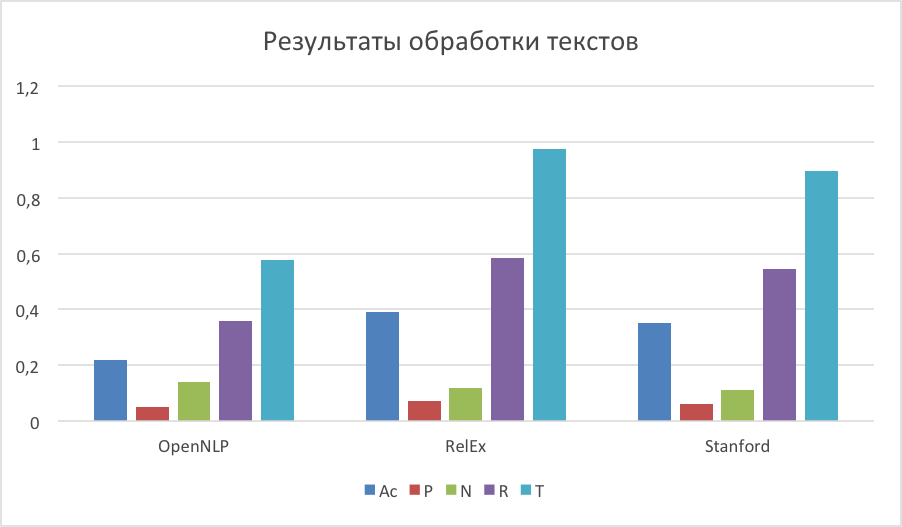
\includegraphics [scale=0.7] {ParserCompare}
  \caption{Результаты анализа средств обработки естественного языка} 
  \label{img:ParserCompare}  
\end{figure}



\begin{longtable}{|p{2cm}|p{4cm}|p{8cm}|}
 \caption[Таблица метрик]{Таблица метрик}\label{Metrics} \\ 
 \hline
 
 \multicolumn{1}{|c|}{\textbf{Метрика}} & \multicolumn{1}{c|}{\textbf{Описание}} & \multicolumn{1}{c|}{\textbf{Формула}} \\ \hline 
\endfirsthead
\multicolumn{2}{c}%
{{\bfseries \tablename\ \thetable{} -- продолжение}} \\
\hline\multicolumn{1}{|c|}{\textbf{Метрика}} & \multicolumn{1}{c|}{\textbf{Описание}} & \multicolumn{1}{c|}{\textbf{Формула}}  \\ \hline 
\endhead
\endfoot

\hline \hline
\endlastfoot
   \hline

Precision	& Точность & 
$$ 
P=\frac{tp}{tp+fp},
$$ где $P$~--- precision, $tp$~---  успешно обработанные слова, $fp$~--- ложно успешные \\
 \hline
Recall	& Чувствительность & 
$$ 
R=\frac{tp}{tp+fn},
$$ где $R$~--- recall, $tp$~--- успешно обработанные слова, $fn$~--- ложно неуспешные \\
 \hline
$F$	& $F$~--- measure (результативность) & 
$$ 
F=\frac{P*R}{P+R},
$$ где $P$~--- precision, $R$~--- recall.   \\

 
\end{longtable}


Кроме того, в главе 1 проведен анализ существующих программных систем автоматизации в области поддержки информационной инфраструктуры предприятия: HP Open View\footnote{\url{https://ru.wikipedia.org/wiki/HP_OpenView}}, ServiceNOW\footnote{\url{http://www.servicenow.com/}}, IBM Watson\footnote{\url{http://www.ibm.com/smarterplanet/us/en/ibmwatson/}}.
Установлено, что все рассмотренные системы не соответствуют полному набору необходимых требований, приведенных во введении. Таблица \ref{Comparsion} содержит сводные данные по рассмотренным системам~--- указаны наличие или отсутствие  у них той или иной функции. Как видно, ни одно из рассмотренных решений не способно проводить логические рассуждения. Наиболее развитой на сегодняшней день программной системой является комплекс IBM Watson.

\begin{longtable}{|p{6cm}|p{0.5cm}|p{0.5cm}|p{0.5cm}|}
 \caption[Сравнительный анализ существующих программных систем.]{Сравнительный анализ существующих программных систем.}\label{Comparsion} \\ 
 \hline
 
 \multicolumn{1}{|c|}{\textbf{Сравнительный пункт}} & \multicolumn{1}{c|}{\textbf{HP Open View}} & \multicolumn{1}{c|}{\textbf{ServiceNOW}} & \multicolumn{1}{c|}{\textbf{IBM Watson}} \\ \hline 
\endfirsthead
\multicolumn{2}{c}%
{{\bfseries \tablename\ \thetable{} -- продолжение}} \\
\hline \multicolumn{1}{|c|}{\textbf{Сравнительный пункт}} & \multicolumn{1}{c|}{\textbf{HP Open View}} & \multicolumn{1}{c|}{\textbf{ServiceNOW}} & \multicolumn{1}{c|}{\textbf{IBM Watson}}  \\ \hline 
\endhead
\endfoot

\hline \hline
\endlastfoot
\hline
   Мониторинг & Да & Да & Да \\
   \hline
   Регистрация инцидентов & Да & Да & Да\\
   \hline
   Управление системами & Да & Нет & Нет \\
   \hline 
   Создание цепи обработки (Workflow) инцидента & Да & Да & Нет \\
   \hline 
   Понимание и формализация запросов на естественном языке & Нет & Нет & Да \\
   \hline 
   Поиск решений & Нет & Нет & Да \\
   \hline 
   Применение решений & Нет & Нет & Нет \\
   \hline
   Обучение & Нет & Нет & Да \\
   \hline
   Умение проводить логические рассуждения: генерализацию, специализацию, синонимичный поиск & Нет & Нет & Нет \\
   
\end{longtable}



%=================
%===Second chapter
%=================

\textbf{Вторая глава} посвящена построению модели интеллектуальной системы принятия решений для регистрации и анализа проблемных ситуаций в ИТ-инфраструктуре предприятия. Рассмотрены три принципиальных подхода к решению проблемы:
 \begin{itemize}
	\item модель Menta 0.1, построенная с использованием деревьев принятия решений;
	\item модель Menta 0.3, построенная с использованием генетических алгоритмов;
	\item модель TU 1.0, основанная на модели мышления Марвина Мински.
\end{itemize} \par

Отметим, что модель, построенная на базе нейронных сетей (поддерживающая обучение), была отброшена на предварительной стадии оценки, так как она предъявляет большие требования к производительности, что в свою очередь порождает высокую стоимость. Далее каждая модель описана подробно.

\textbf{Модель Menta 0.1, построенная с использованием деревьев принятия решений}, была одной из первых, которая была опробована. При построении модели использованы следующие компоненты: обработка запросов на естественном языке; поиск решения; применение решения. \par
Система ориентирована на выполнение простых команд, например, «добавить поле в форму». В целом работа системы характеризуется следующим алгоритмом:
\begin{enumerate}
	\item получение и формализация запроса;
	\item поиск решения при помощи деревьев принятия решений;
	\item изменение модели приложения в формате OWL;
	\item генерация и компиляция приложения.
\end{enumerate} \par
В результате экспериментов было выявлено отсутствие устойчивости к ошибкам входной информации: грамматическим и содержательным. Например, входной файл не имел отношения к программной системе, модель которой содержалась в базе знаний; система поиска решения работала только в рамках модели одной программы;  отсутствовала функция обучения. \par



\textbf{Модель Menta 0.3, построенная с использованием генетических алгоритмов}.
В данную модель по сравнению с предыдущей были добавлены модуль логики для оценки решения и модуль генетических алгоритмов для генерации решения. В рамках модели Menta 0.3 были отработаны следующие основные компоненты будущей итоговой модели: критерии приемки (Acceptance Criteria); How-To~--- для хранения решений проанализированных проблем; формат данных OWL; использование логических вычислений для проверки решения. Система Menta 0.3 содержала, как составляющую часть, модель целевого приложения (как и Menta 0.1) и список решений тех или иных проблем (How-To), найденных ранее. При помощи генетического алгоритма модель строила решение, проверяла его при помощи логического движка NARS\footnote{\url{http://www.cogsci.indiana.edu/farg/peiwang/papers.html}} на соответствие критериям, заданным пользователем. С точки зрения генетических алгоритмов, такая проверка~--- функция отбора особей из поколения.  \par
В результате проведенных экспериментов были выявлены следующие проблемы: отсутствие обучения; отсутствие обработки естественного языка; после апробации оказалось, что список критериев соответствия решения требованием пользователя (набор правил) практически описывают необходимое решение (то, которое должно быть найдено), что являлось недопустимым. \par


\textbf{Модель TU 1.0, основанная на модели мышления Марвина Мински}, была построена с применением известной теории Марвина Мински\footnote{\url{https://en.wikipedia.org/wiki/The_Emotion_Machine}}, сохранила следующие основные концептуальные элементы предыдущих моделей и показала свою состоятельность на контрольных примерах: Acceptance Criteria; обучение; поиск и применение решения; отсутствие обработки естественного языка. Данная модель является более универсальной и представляет собой верхнеуровневую архитектуру обработки запроса (мышления), где компонентами являются лучшие по функциональности компоненты предыдущих систем. Реализованная модель названа TU (от англ. "Thinking Understanding\"~~--- «мышление и понимание»). \par
Одним из основных компонентов системы TU является триплет \triplet\ (далее \tripletshort), схематичное изображение которого представлено на рисунке \ref{img:csw}. Критик реагирует, Селектор выбирает ресурс, Образ мышления выполняет работу.
\begin{figure} [h] 
  \center
  \includegraphics [scale=1.0] {CSW}
  \caption{\tripletshort} 
  \label{img:csw}  
\end{figure}


\emph{Критик} представляет собой определенный переключатель, который срабатывает при определенных событиях. Например, «включился свет, и зрачки сузились», «обожглись и одернули руку». Критик активируется только тогда, когда для этого достаточно обстоятельств. Одновременно может активироваться несколько критиков. Например, человек решает сложную задачу, идет активация множества критиков: выполнить расчет, уточнить технические детали. Кроме того, параллельно может активироваться критик контроля уровня загруженности, сообщающий о необходимости отдыха.\par
\emph{Селектор} занимается выбором необходимых ресурсов, которыми, например, могу быть: критик, образ мышления. \par
\emph{Образ мышления}~--- это способ решения проблемы. Он может быть сложным и, например, может активировать других критиков. Так, размышляя над проблемой, специалист понимает, что нужно рассмотреть все возможные комбинации, и тут он решает поискать готовое решение: может быть кто-то уже рассмотрел все возможные комбинации, и можно будет его использовать. Здесь «поиск готового решения» является критиком внутри образа мышления «поиск решения».\par

На рисунке \ref{img:csw_ex} представлена расширенная модель работы \tripletshort. Критик активирует селектор, который возвращает ресурс образ мышления (кругами отмечены различные ресурсы: критики, селекторы, образы мышления \etc). Последний в свою очередь может активировать нового критика или же совершить определенные действия. Например, появилась проблема, связанная с отсутствием доступа, значит, нужно запустить служебную программу для предоставления прав пользователю. Под ресурсами здесь понимается набор знаний из базы знаний: критики, селекторы, образы мышления, готовые решения. \par
Если активировалось много критиков, то проблему нужно уточнить, иначе степень неопределенности будет слишком высокой. Если проблема очень похожа на уже проанализированную, то можно действовать и судить по аналогии. \par
\begin{figure} [h] 
  \center
  \includegraphics [scale=0.6] {CSW_EX}
  \caption{\tripletshort\ в разрезе ресурсов} 
  \label{img:csw_ex}  
\end{figure}
Другой важной частью теории Мински являются уровни мышления. Эта концепция распределяет активность мышления между 6-ю уровнями: чем выше уровень, тем сильнее активность. В Таблице \ref{ThinkingLevelDescription} представлено описание уровней мышления с примерами. \par
На этом исследование моделей мышлений было завершено и были сделаны выводы, основные из которых состоят в следующем. 

\begin{table} [htbp]
  \centering
  \parbox{15cm}{\caption{Описание шести уровней мышления, заложенных в модель Мински}\label{ThinkingLevelDescription}}
%  \begin{center}
  \begin{tabular}{| p{5cm} | p{11cm} |}
  
  \hline
\textbf{Уровень} & \textbf{Описание} \\
  \hline
  
Инстинктивный уровень & Происходят инстинктивные реакции (врожденные). Например, коленный рефлекс. Общую формулу для этого уровня можно выразить как «если ..., то сделать так» \\
  \hline

Уровень обученных реакций & Используются накопленные знания, то есть те знания, которым человек обучается в течение жизни. Например, переходить дорогу на зеленый свет. Общую формулу для этого уровня можно описать как «если ..., то сделать так» \\
  \hline

Уровень рассуждений & Мышление с использованием рассуждений. Например, если перебежать дорогу на зеленый свет, то можно успеть вовремя. На данном уровне сравниваются последствия нескольких решений и выбирается оптимальное. Общую формулу для этого уровня можно выразить как «если ..., то сделать так, тогда будет так» \\
  \hline

Рефлексивный уровень & Рассуждения с учетом анализа прошлых событий. Например, «в прошлый раз я побежал на моргающий зеленый и чуть не попал под машину» \\

  \hline
  Саморефлексивный уровень & Построение определенной модели, с помощью которой идет оценка своих поступков. Например, «мое решение не пойти на это собрание было неверным, так как я упустил столько возможностей, я был легкомысленным» \\
  \hline
  Самосознательный уровень & Оценка своих поступков с точки зрения высших идеалов и оценок окружающих. Например, «а что подумают мои друзья? А как бы поступил мой герой?» \\
  \hline
  
  \end{tabular}
%  \end{center}
\end{table}


Для программной экспертной системы очень важно обладать способностью мыслить и рассуждать, например, действовать по аналогии. Множество запросов типично, запросы отличаются лишь параметрами. Например, таковым является запрос «пожалуйста, установите Office, Antivirus» \etc\ Также для экспертной системы важно уметь абстрагировать специализированные рецепты решения. Например, система научилась разрешать инцидент "Please install Firefox"\comma\ абстрагировав данный инцидент до степени "Please install browser"\comma\ система сможет тем же способом устранить проблему "Please install Chrome"\comma\ так как концепции "Firefox"\ и "Chrome"\ связаны через концепцию "Browser". \par
После рассмотрения нескольких моделей была выбрана модель мышления Марвина Мински, так как она наиболее соответствует целевой области поддержки ИТ-инфраструктуры предприятия. На основе подхода Мински построена модель системы, которая реализует основные функции: обучение, понимание инцидента, поиск решения, применение решения. 


%=================
%===3rd chapter
%=================
В \textbf{третьей главе} описаны архитектура и реализация системы, основанной на модели Thinking Understanding (TU).
Архитектура представляет собой модули. Основные компоненты системы описаны в Таблице \ref{MainComponents}. Система может функционировать в режиме обучения и в режиме устранения проблемных ситуаций. 
\begin{longtable}{|p{7cm}|p{8cm}|}
 \caption[Основные компоненты системы Thinking Understanding]{Основные компоненты системы Thinking Understanding}\label{MainComponents} \\ 
 \hline
 
 \multicolumn{1}{|c|}{\textbf{Компонент}} & \multicolumn{1}{c|}{\textbf{Описание}}  \\ \hline 
\endfirsthead
\multicolumn{2}{c}%
{{\bfseries \tablename\ \thetable{} -- продолжение}} \\
\hline \multicolumn{1}{|c|}{\textbf{Компонент}} &
\multicolumn{1}{c|}{\textbf{Описание}}  \\ \hline 
\endhead

\endfoot

\hline \hline
\endlastfoot
\hline
   TU Webservice & Основной компонент взаимодействия со внешними системами, включая пользователя \\
   \hline
   CoreService & Ядро системы, содержит основные классы\\
   \hline
   DataService & Компонент работы с данными \\
   \hline 
   Reasoner & Компонент вероятностной логики \\
   \hline 
   ClientAgent & Компонент выполнения скриптов на целевой машине \\
   \hline 
   MessageBus & Шина данных для системы \\
    
\end{longtable}
В главе 3 приведено детальное описание всех компонентов и подкомпонентов. Для лучшего понимания представлены описание механизма взаимодействия компонентов и общий сценарий использования системы.
%Каждый пункт, подпункт и перечисление записывают с абзацного отступа (ГОСТ 2.105-95, 4.1.8)

\begin{enumerate}
	\item Поступает запрос от пользователя: 
	"User had received wrong application. User has ordered Wordfinder Business Economical. However she received wrong version, she received Wordfinder Tehcnical instead of Business Economical. Please assist"\ («Пользователь получил неверное приложение. Пользователь заказал приложение "Wordfinder. Бизнес версия"\,, но получил неверную версию,~--- "Wordfinder. Техническая версия". Пожалуйста, помогите»);
	\item Компонент GoalManger (Менеджер целей) устанавливает цель системы HelpUser (Помочь пользователю);
	\item Главный компонент Thinking Life Cycle (далее TLC) активирует набор компонетов Critic (Критик), привязанный к данной цели (HelpUser); 
	\item Активируется компонент PreliminaryAnnorator (Предварительный обработчик), который разбирает запрос, проводя орфографическую коррекцию и предварительный разбор;
	\item Компонент KnowledgeBaseAnnotator (разбор при помощи накопленных знаний) создает семантическую сеть и ссылки на нее;
	\item Компонент Critic (Критик), привязанный к цели HelpUser на Рефлексивном уровне, запускает WayToThink (Образ мышления) ProblemSolving (Разрешить проблемную ситуацию) с целью: ResolveIncident;
	\item Компонент Critic на Рефликсивном уровне выбирает WayToThink KnowingHow (Поиск рецепта решения);
	\begin{enumerate}
	\item Запускаются параллельно все компоненты класса Critic, которые привязаны к цели ResolveIncident (Решить проблему), в данном случае это DirectInstruction (прямые инструкции), ProblemWithDesiredState (проблемы с желаемым состоянием), ProblemWithoutDesiredState (проблема без желаемого состояния);
	\item Компонент Selector (Селектор) выбирает среди всех результатов наиболее вероятный результат работы. В данном случае им будет Problem Description with desired state (Проблема с желаемым состоянием);
	\item Компонент KnowingHow сохраняет варианты выбора Selector;
	\item Компонент Simulation (Моделирование) WayToThink с параметрами «создать модель текущий ситуации» создает: концепцию существующей ситуации (CurrentState), концепцию пользователя, концепцию программного обеспечения;
	\item Компонент Reformulation WayToThink (Компонент дополнения), используя результаты предыдущего шага, синтезирует артефакты, которых не хватает, чтобы получить из CurrentState DesiredState (Желаемое состояние), так как он не указан явно. WayToThink запускает Critic размышления, чтобы найти корень проблемы. Он находит CurrentState (настоящее состояние)~--- Wordfinder Tehcnical и DesiredState (состояние, которое нужно пользователю)~--- Wordfinder Business Economical;
	\item Рефлексивные Critic оценивают состояние системы~--- на каком шаге она находится, и если цель не достигнута, то запускают другой WayToThink, например, DirectInstruction;
	\item Компонент Critic Solution Generator (Компонент генерации решения) запускает KnowingHow WayToThink, ExtensiveSearch (Поиск решения);
	\item Компонент Selector выбирает наиболее вероятный образ мышления. В данном случае это будет ExtensiveSearch, который будет находить решения, позволяющие привести систему в необходимое пользователю состояние (DesiredState), если сделать это невозможно, то система инициирует коммуникацию с пользователем. 
 \end{enumerate}
	 \item Рефлексивный Critic проверяет состояние системы. Если Цель достигнута, то пользователю посылается ответ, информирующий об этом.
	 \item На данном шаге активируются компоненты класса Critic на cамосознательном уровне, которые сохраняют информацию о затратах на решение.
  \end{enumerate}\par
Для работы системы создана уникальная модель данных~--- TU Knowledge, которая сочетает в себе OWL и графовую базу данных. Язык OWL, появившийся для структурирования информации в Вебе, обрел широкое использование во многих схемах данных, так как дал возможность дополнительного расширенного описания взаимосвязи между данными. 

%=================
%===4 chapter
%=================
В \textbf{главе 4} приведены результаты оценки эффективности работы модели, полученные на основе проведенных экспериментов.
 Были проведены тесты для выполнения сравнения с работой специалиста-человека. Был выбран контрольный список запросов пользователя (инцидентов). Сравнивалась скорость разрешения инцидента. Основное время при опросе специалиста тратилось на коммуникацию. В таблице \ref{HumanComparison} приведены результаты сравнения. Тесты были выполнены на компьютере Intel Core i7 1700 MHz, 8GB RAM, 256 GB SSD, FreeBSD. Из результатов видно, что система работает так же или лучше, чем специалист технической поддержки.
\begin{longtable}{|p{12cm}|p{2cm}|p{2cm}|}
 \caption[Результаты сравнения с работой специалиста]{Результаты сравнения с работой специалиста технической поддержки}\label{HumanComparison} \\ 
 \hline
 
 \multicolumn{1}{|c|}{\textbf{Инцидент}} & \multicolumn{1}{c|}{\textbf{TSS1 (.мс)}} & \multicolumn{1}{c|}{\textbf{TU (.мс)}}  \\ \hline 
\endfirsthead
\multicolumn{2}{c}%
{{\bfseries \tablename\ \thetable{} -- продолжение}} \\
\hline
\multicolumn{1}{|c|}{\textbf{Инцидент}} & \multicolumn{1}{c|}{\textbf{TSS1 (.мс)}} & \multicolumn{1}{c|}{\textbf{TU (.мс)}}  \\ \hline 
\endhead

\endfoot

\hline \hline
\endlastfoot
\hline
  Tense is kind of concept~(Время~--- это концепция) & 15000 & 385 \\
  
  \hline
  Please install Firefox~(Установите Firefox)   & 9000 & 859 \\
  \hline
  Browser is an object~(Браузер~--- это объект)   & 20000 & 400 \\
  \hline
  Firefox is a browser~(Firefox~--- это браузер)   & 5000 & 659  \\
  \hline
  Install is an action~(Установить~--- это действие)   & 8000 & 486 \\
  \hline
  User miss Internet Explorer 8~(У пользователя нет Internet Explorer 8).     & 10000 & 10589 \\
  \hline
  User needs document portal update~(Пользователю требуется обновление документов)    & 15000 & 16543 \\
  \hline
  Add new alias Host name on host that alias is wanted to: hrportal.lalala.biz IP address on host that alias is wanted to: 322.223.333.22 Wanted Alias:    webadviser.lalala.net~(Добавьте, пожалуйста, новую ссылку на hrportal.lalala.biz через 322.223.333.22)    & 10000 & 18432  \\ 
  \hline
  Outlook Web Access (CCC)~--- 403~--- Forbidden: Access is denied~(Нет доступа к Outlook Web Access (CCC)). & 15000 & 10342\\ 
  \hline
  PP2C~--- Cisco IP communicator. Please see if you can fix the problem with the ip phone, it's stuck on configuring ip + sometimes Server error rejected: Security etc~(PP2C~--- коммуникатор Cisco IP. Пожалуйста, помогите исправить проблему с ИП-телефоном, он застревает во время конфигурирования и иногда показывает ошибку «Безопасность»)  & 13000 & 12343 \\ 
   
  \end{longtable}
  
  Показатели, приведенные во введении, приобрели следующие значения $T_qp$=32,9 при n=8; SLA=0,96; $\alpha$=0,04;  $\alpha_n$=2920. 

%=================
%===Conclusion
%=================
В \textbf{заключении} диссертации приведены основные выводы по работе:
%% Согласно ГОСТ Р 7.0.11-2011:
%% 5.3.3 В заключении диссертации излагают итоги выполненного исследования, рекомендации, перспективы дальнейшей разработки темы.
%% 9.2.3 В заключении автореферата диссертации излагают итоги данного исследования, рекомендации и перспективы дальнейшей разработки темы.

Решены следующие задачи и достигнуты следующие результаты.
\begin{enumerate}
  \item Создана модель проблемно-ориентированной системы управления, принятия решений в области обслуживания информационной структуры предприятия на основе модели мышления;
  \item Представлены новая модель данных для модели мышления и оригинальный способ ее хранения, эффективный по сравнению с другими базами данных;
  \item Выполнено оригинальное исследование моделей мышления в области обслуживания информационной структуры предприятия;
  \item На основе модели созданы архитектура системы и ее прототип; 
  \item Созданы специальные алгоритмы для анализа запросов пользователей и принятия решений;
  \item Система, разработанная в рамках данной работы, включает в себя инновационные методы и алгоритмы поддержки принятия решений, использует модель мышления на базе модели мышления Мински;
  \item Представлена наглядная визуализация структуры области удаленной поддержки инфраструктуры.
\end{enumerate}

Представленные в диссертации модель мышления, ее архитектура и реализация являются уникальными~--- на данный момент времени это единственная реализация модели мышления Мински. \par
Система, разработанная в диссертации, не является узкоспециализированной. Она также подходит для других областей, где требуется поддержка принятия решений. Например, при постановке медицинского диагноза, чтобы отбросить ложные диагнозы. \par
Кроме того, в систему можно загрузить данные о взаимосвязи органов человека и болезней. Далее, к каждому заболеванию добавить симптом и способ лечения, после этого можно делать запрос с симптомами, и система выдаст список вероятных заболеваний со способами их лечения. \par
В области диагностики проблем можно обучить систему узлам автомобиля, проблемам, с ними связанными, признаками этих проблем и способами их устранения. 





 

%\newpage
\renewcommand{\refname}{\large Публикации автора по теме диссертации}

%\insertbiblioauthor                          % Подключаем Bib-базы
\insertbiblioall

